\chapter{Hardware}

\section{Circuit of the TransistorTester}
\label{sec:hardware}
The circuit of the TransistorTester in figure \ref{fig:ttester} is based on the circuit of
 Markus F. released in Abb.~1 of AVR-Transistortester report \cite{Frejek}.
Changed or moved parts are marked with green color, optional parts are marked with red color.

Some changes are made because the electronical power switch make problems in some implementations.
Therefore the resistor R7 is reduced to \(3.3k\Omega\). The capacitor C2 is reduced to
10nF and R8 is moved so that the PD6 output does not try to switch the C2 capacitor directly.
 Additional blocking capacitors are added and should be placed
near the power connection of the Atmega and near the Voltage regulator.

Because the PD7 input and PC6 (RESET) are the only pins, where pull up resistors where
needed, one extra \(27k\Omega\) resistor is added to the PD7 (pin~13) input. With this modification
the software can disable all internal pull up resistors of the ATmega.

The additional crystal with its 22pF capacitors are optional added. 
The accuracy of a crystal has the benefit of more stable time measurement for getting the
capacitor values.

New software version can use a voltage scale switch of the ADC. The speed of switching is reduced
by the external capacitor C1 at the AREF (21) pin of the ATmega. To avoid slowing down the
measurement speed more than necessary, the value of this capacitor should be reduced to 1nF.
Removing of the capacitor C1 is also possible.
For adapting the software to the actual circuit take a look to the Makefile options in the
configuring chapter \ref{sec:config} at page~\pageref{sec:config}.

Some different versions of R11 / R12 resistor combinations circulates
in the internet. I~have adapted my software to the original of Markus F. \cite{Frejek} with \(10k\Omega\) and \(3.3k\Omega\).
The voltage ration of the divider can be set with Makefile options.

The additional 2.5V precision voltage reference connected at pin PC4 (ADC4) can be used to
check and calibrate the VCC voltage, but is not required. You can use a LM4040-AIZ2.5 (0.1\%),
a LT1004CZ-2.5 (0.8\%) or a LM336-Z2.5 (0.8\%) as voltage reference.
If you don't install the precision voltage reference and you don't add the relay extension,
you should install a pull up resistor R16 to PC4 with a higher resistance value (\(47k\Omega\)).
This helps the software to detect the missing voltage reference.
A optional ISP connector has been added to easier load new software versions to the tester.

\begin{figure}[H]
\centering

\includegraphics[width=18cm]{../FIG/ttester.eps}
\caption{New circuit of TransistorTester}
\label{fig:ttester}
\end{figure}
The software can follow to another pin assignment of port D for a simpler connection of the
LCD display. 
The following table \ref{tab:grid-change} shows the modifies assignments for the strip grid layout and
the connection of a graphical display for the micocontrollers ATmega8/168/328.
Also the using of port inputs for additional functions is shown.
With the connections for the graphical display with the strip grid option (STRIP\_GRID\_BOARD)
the frequency counter function can not be used, because the port PD4 (T0) is used.
But this connection is used by a chinese version with graphical display. 



\begin{table}[H]
  \begin{center}
    \begin{tabular}{| c || c | c | c | c | c | c |}
    \hline
           & character  & char. LCD    & ST7565     & ST7565       & SSD1306     & additional function \\
      Port &   LCD      & STRIP\_GRID  &   LCD      & STRIP\_GRID  &   I\textsuperscript{2}C       & \\
    \hline
    \hline
    PD0    &  LCD-D4    &  pushbutton  &  LCD-REST    &            &           & \\
    \hline
    PD1    &  LCD-D5    &  LCD-D7      &  LCD-RS      & LCD-SI     &           &  rotary encoder 2  \\
    \hline
    PD2    &  LCD-D6    &  LCD-D6      &  LCD-SCLK    & LCD-SCLK   &  LCD-SDA  & \\
    \hline
    PD3    &  LCD-D7    &  LCD-D5      &  LCD-SI      & LCD-A0 (RS) &           & rotary encoder 1 \\
    \hline
    PD4    &  LCD-RS    &  LCD-D4      &              & LCD-REST    &           & frequency counter \\
    \hline
    PD5    &  LCD-E     &  LCD-E       &              &             &  LCD-SCL  & \\
    \hline
    PD7    & pushbutton &  LCD-RS      &              &             &           &  \\
    \hline
    \end{tabular}
  \end{center}
  \caption{Different variations of the display port assignments}
  \label{tab:grid-change}
\end{table}

\section {Extensions for the TransistorTester}

\subsection{Protection of the ATmega inputs}

For better protection of the ATmega inputs one of the additional circuits~ \ref{fig:relay_addon} 
can be integrated. The de-energized contacts of the relay protect the ATmega without power.
The contacts will be opened by software only for measurement.
Also with the additional diode protection the chance of the ATmega will be better to survive the connection
of a capacitor with higher residual voltage.
A complete protection is not possible. Therefore capacitors should always be discharged before measuring.

\begin{figure}[H]
  \begin{subfigure}[b]{9cm}
    \centering
    
\includegraphics[width=7cm]{../FIG/relay_addon.eps}
    \caption{with Relay}
  \end{subfigure}
  ~
  \begin{subfigure}[b]{9cm}
    \centering
    
\includegraphics[width=7cm]{../FIG/diode_addon.eps}
    \caption{with Diodes}
  \end{subfigure}
  \caption{Additional protection of the ATmega inputs}
  \label{fig:relay_addon}
\end{figure}

\subsection{Measurement of zener voltage above 4 Volt}

If the serial output of text is not required, the Pin PC3 of the ATmega can be used as analog
input for measuring a external voltage. The voltage can be up to 50V with the optional 10:1 resistor
divider and can be used for measuring the breakdown voltage of a zener diode. 
A current limiting power supply with up to 50V can be switched on with low signal at PD7 pin of the
ATmega to deliver current for testing the break down voltage of a zener diode.
Figure~\ref{fig:zener} shows a suggestion for this expansion.
The tester shows the external voltage as long as you hold the key pressed.
About 40mA more battery current is used by this expansion during key pressing.

\begin{figure}[H]
\centering

\includegraphics[width=12cm]{../FIG/zener_exp.eps}
\caption{Expansion for measuring of break down voltage of Zener diodes}
\label{fig:zener}
\end{figure}

The 10:1 voltage divider can be used with the optional dialog part for the ATmega328 without the 
activated DC-DC converter for the zener diode measurement.
Without the pressed key the voltage converter is not powered. For that the external voltage 
(for example battery voltage) can be measured at the zener diode port.
You can only measure positiv DC voltages up to 50V.
You have also to respect the correct polarity.

\subsection{Frequency generator}

With the dialog part of the ATmega you can also select a frequency generator, which supports
currently a selection of frequencies from \(1 Hz\) up to \(2 MHz\).
The output of the 5V signal is done with a \(680\Omega\) resistor to test port TP2.
You can use the GND signal from the minus pin of the zener diode extension or the test port TP1.
The test port TP3 is connected to GND with a \(680\Omega\) resistor.
Of course you can also connect a driver circuit to the ATmega port PB2 with a separate output
driver circuit and a additional output terminal. But the input of this circuit should not insert a
big capacity load for the ATmega output.

\subsection{Frequency measurement}
\label{sec:frequency_counter}

For using the with the dialog selectable frequency measurement is a little hardware extension
necessary. The input pin PD4 (T0/PCINT20) of the ATmega is used for the frequency measurement.
The same pin is also used for the connection of the LCD. With normal layout, the PD4 pin is connected
to the LCD-RS signal, with the strip grid design it is connected to LCD-D4.
For both signals the PD4 pin can be switched to input as long as no output to the LCD is
required. The LCD respect the input value only, if the LCD-E signal is switched to GND.
For driving the input pin from external clock source at least one serial resistor of \(270\Omega\) should be used.
Better you should use the circuit of figure~\ref{fig:FreqMes} .
The voltage at the PD4 pin (LCD-RS or LCD-D4) should be adjusted to \(2.4V\) without the assembled ATmega
or during frequency measurement of the ATmega, to get the best sensivity for the input frequency signal.
The LCD should always be installed for adjusting, because the pull up resistor of the LCD change the voltage.

\begin{figure}[H]
\centering

\includegraphics[width=7cm]{../FIG/Frequency_addon.eps}
\caption{Extension for measurement of frequency}
\label{fig:FreqMes}
\end{figure}

\subsection{Using of a rotary pulse encoder}

For easier control of the menu function for the ATmega328 you can expand the circuit 
by a rotary pulse encoder with a push button.
The circuit~\ref{fig:RotExt} shows a standard expansion for a normal character LCD.
All signals for the connection of the rotary pulse encoder are available at the plug connector
for the LCD. For this reason the expansion can also be easy upgraded for many existing testers.
In many cases the graphical LCD is assembled on a adapter board with some connection pins
of the character LCD. Also in this cases the upgrade with a rotary encoder is not very difficult to do.

\begin{figure}[H]
\centering

\includegraphics[width=6cm]{../FIG/rotary_extension.eps}
\caption{Expansion with a rotary pulse encoder}
\label{fig:RotExt}
\end{figure}

The figure~\ref{fig:RotEnc} shows the feature of two different rotary pulse encoder.
The version 1 has twice as much indexed positions (detents) per turn as pulses per turn.
The version 2 has the same count of detents as pulses per turn.
The slope of one of the two switch signals is sometimes exactly at the detent of the 
rotary pulse encoder.

\begin{figure}[H]
\centering

\includegraphics[width=14cm]{../FIG/rotary_encoder.eps}
\caption{Feature of two different rotary pulse encoder}
\label{fig:RotEnc}
\end{figure}

The figure~\ref{fig:RotBounce} shows a rotary pulse encoder, which has not only
bouncing contacts, but also has a unstable state of one of the switches at the indexed
position (detent). Every change of the state of the switches is detected by the program
and saved in a cyclic buffer. Therefore the last three states of the switches can be checked
after every status change.
For every cycle of switch states a total of four sequences of state can be defined for every direction of rotation.
If there is only one indexed position (detent) for every cycle of switch states, only
one of the state sequence pair must be monitored (WITH\_ROTARY\_SWITCH=2 or 3) for correct counting.
If there are two indexed positions for every cycle of the switch states, as shown in figure~\ref{fig:RotBounce},
you must monitor two pairs of switch state sequences (WITH\_ROTARY\_SWITCH=1).
You can choise any resolution for the WITH\_ROTARY\_SWITCH for a rotary pulse encoder without
indexed positions. A value of 2 or 3 selects the lowest resolution, 1 selects a middle resolution
and 5 selects the highest resulution.
A oscillation of the selection (counter up, counter down) can be avoided with the type of monitoring,
but sometimes a count can be missed with a bad placement of the indexed position.

\begin{figure}[H]
\centering

\includegraphics[width=14cm]{../FIG/rotary_bouncing.eps}
\caption{A rotary pulse encoder with bouncing switches}
\label{fig:RotBounce}
\end{figure}

In place of the two switches of a rotary switch encoder you can also install two seperate
key buttons for Up and Down movement, if no rotation switch encoder is present or favored.
In this case the option WITH\_ROTARY\_SWITCH must be set to 4 for a correct handling of
the program.

\subsection{Connection of a graphical display}

Many thanks to Wolfgang Sch. for his work to support a chinese version with ST7565 controller.
By now you can also connect a graphical 128x64 pixel LCD with a ST7565 controller.
Because the ST7565 controller is connected with a serial interface, only four signal
lines are required. Two port D pins of the ATmega can be used otherwise.
The ATmega processor should have at least 32k flash memory for the support of a graphical display.
The ST7565 controller works with a operating voltage of 3.3V .
Therefore a additional 3.3V voltage regulator is required.
The data sheet of the ST7565 controller does not allow the direct connection of input pins to
5V signal level. So the extension of figure \ref{fig:ST7565lcd} uses a additional 74HC4050 CMOS
device for the conversion of the voltage level.
You can try to exchange the four 74HC4050 gates with four resistors of about \(2.7k\Omega\).
With the voltage drop at the resistors you will prevent the increase of the 3.3V controller power voltage 
across the diodes of the controller inputs from the 5V ATmega outputs signals.
You have to try, if the signal form with the resistors can be accepted from the ST7565 controller inputs.
The signal form at the controller inputs will be more simular to the output shape of the ATmega with the 74HC4050 gates in any case.\\

\begin{figure}[H]
\centering

\includegraphics[width=14cm]{../FIG/ST7565lcd.eps}
\caption{Connection of a graphical display with ST7565 controller}
\label{fig:ST7565lcd}
\end{figure}

Normally the ST7565 or SSD1306 controller is connected with a 4-wire SPI interface.
But with the SSD1306 controller you can also use a I\textsuperscript{2}C interface with PD2 as SDA and PD5 as SCL signal.
The SDA and SCL signals must be equipped with pull-up resistors of about \(4.7k\Omega\) to 3.3V.
A solution for connecting the OLED display shows the figure  \ref{fig:ssd1306i2c}.
The outputs of the ATmega is only switched to 0V for the I\textsuperscript{2}C signals.
Before connecting the pull-up resistors to 5V you must check, if your display module can tolerate
a 5V signal level. Normally the data inputs of the controller are protected with diodes to 3.3V.
You should make shure, that you have loaded a program with the I\textsuperscript{2}C support to the ATmega 
before the Display is connected. If you have loaded a program with another interface, 
the output are also switched to the 5V side.
Because I have determined a influence to the tester results across the VCC connection of a OLED module,
a additional decoupling with a serial resistor of \(68~\Omega\) with a additional \(10~\mu\) blocking capacitor
is recommended. Instead of the \(68~\Omega\) resistor you can also use a inductor with about \(1~mH\).
Without the additional filter my tester has reported collector residual currents with bipolar transistors and a
OLED display.
Also you should check the pin sequence of your OLED module, some moduls have a different location of GND and VCC.
 
\begin{figure}[H]
\centering

\includegraphics[width=14cm]{../FIG/SSD1306_I2C.eps}
\caption{Connection of a graphical OLED display with I\textsuperscript{2}C interface}
\label{fig:ssd1306i2c}
\end{figure}

For connection to the ATmega644 series of processors the pins PB2 to PB5 instead of PD0 to PD3 are used.
The exchange of a text display to a graphical display is possible with a adapter printed board because
all required data signals and power signals are available at the LCD connector.
A little simpler is the connection of a graphical display with a ST7920 controller because
the controller can operate with 5V power voltage.
For that the display should offer 128x64 visible pixels.
The display module with the ST7920 controller can be connected with the 4-bit parallel interface or with a
special serial interface., as shown in figure \ref{fig:ST7920lcd}.
 
\begin{figure}[H]
\centering

\includegraphics[width=14cm]{../FIG/ST7920interface.eps}
\caption{Connection of a display with ST7920 controller}
\label{fig:ST7920lcd}
\end{figure}

For both connection types the software must be configured in a special way.
The Makefile option ''WITH\_LCD\_ST7565 = 7920'' must be set in any case, for the serial
connection type you must set also the option ''CFLAGS += -DLCD\_INTERFACE\_MODE=5''.
The orientation of the presentation can be changed with the options LCD\_ST7565\_H\_FLIP and 
LCD\_ST7565\_V\_FLIP in the same way as with the other graphical displays.

A special case is the connection of displays with a ST7108 controller. Because these displays can only use 
the 8-bit parallel interface, you must use a serial to parallel converter.
The simplest way seems to be the use of a 74HCT164 or a 74HCT595 chip.
A suitable suggestion of a connection circuit shows the figure \ref{fig:ST7108lcd} .

\begin{figure}[H]
  \begin{subfigure}[b]{9cm}
    \centering
    
\includegraphics[width=8cm]{../FIG/ST7108serial164.eps}
    \caption{with 74HCT164}
  \end{subfigure}
  ~
  \begin{subfigure}[b]{9cm}
    \centering
    
\includegraphics[width=8cm]{../FIG/ST7108serial595.eps}
    \caption{with 74HCT595}
  \end{subfigure}
  \caption{Connection of a graphical display with a ST7108 controller}
  \label{fig:ST7108lcd}
\end{figure}

You must check the pin layout of your LCD module, some moduls have different signal sequence.
Some different pin layouts found in data sheets for the ABG128064 series are shown in table~\ref{tab:ST7108types}.

\begin{table}[H]
  \begin{center}
    \begin{tabular}{| c || c | c | c | c |}
    \hline
           & 128064H  &  128064G  & 128064C  & 128064B \\
    Signal &         &          &         &         \\
    \hline
    \hline
  VDD (5V) &   1     &  2       &   4     & 2       \\
    \hline
  VSS (GND) &   2     &  1       &   3     & 1       \\
    \hline
 VO (Drive) &   3     &  3       &  (5)    & 3       \\
    \hline
  DB0-DB3   &   4-7   &  7-10    &   9-12  & 7-10    \\
    \hline
  DB4-DB7   &   8-11  &  11-14   &   13-16 & 11-14   \\
    \hline
  CS1       &   12    &  15      &   1     & 15      \\
  CS2       &   13    &  16      &   2     & 16      \\
    \hline
  Reset     &   14    &  17      &   -     & 17      \\
    \hline
  R/W       &   15    &  5       &   7     & 5       \\
    \hline
  RS        &   16    &  4       &   6     & 4       \\
    \hline
  E         &   17    &  7       &   8     & 6       \\
    \hline
  VEE       &   18    &  18      &   -     & 18      \\
    \hline
  LEDA      &   19    &  19      &   17    & (19)      \\
  LEDK      &   20    &  20      &   18    & -      \\
    \hline
    \end{tabular}
  \end{center}
  \caption{Pin layout of different ST7108 moduls}
  \label{tab:ST7108types}
\end{table}


\section{Hints for building the TransistorTester}
Every LCD-display with at least 2x16 character and a HD44780 compatible controller
can be used with the TransistorTester. You should respect the current needed for
illumination, some LCD need lower current than others.
I had tried OLED type displays, but this type cause interference with measurements
of the ATmega and are {\bf not} recommended. Also loading of special characters
for displaying the resistor symbol has caused problems with the OLED.

The resistors R1 to R6 are critical for measurements and this \(680\Omega\) and
\(470k\Omega\) resistors should be measurement type resistors (tolerance of 0.1\%) to
get the full accuracy.
You should use a precision socket for the ATmega microcontroller to enable
the replacement of the microcontroller.
The microcontroller ATmega8, ATmega168 and ATmega328 can be used.
Recommended is a ATmega328, if you wish to use all features.

Anyway you should assemble all parts to printed board without the microcontroller.
A up-to-date low voltage drop regulator like MCP1702-5002 is recommended as IC2, because it
need only \(2\mu A\) of standby current and can still deliver 5V, if your input
voltage is only 5.4V. But this part is not pin compatible to well known 78L05 with TO92 body!

After checking, that all needed parts are at the correct place, you should
first connect the battery or power supply to the printed board without LCD-display
and microcontroller. You should check the voltage at the power pins of the
microcontroller and LCD-display terminal during the Test key is pressed.
The voltage should disappear, if you release the Test key.
If the voltage had correct polarity and value,
you should disconnect the power and assemble the microcontroller with correct
alignment. Be careful and make shure, that all pins of the microcontroller
are in the socket holes.
Now you can also connect the LCD. Check if power pins of the LCD has the right connection to
GND and VCC of your board.

If you are shure that everything is all right, reconnect the power. 
If you have already programmed the ATmega, you can press the Test button.
By pressing the Test key, the background light of the LCD should switch on.
If you release the Test button, the LED should illuminate weak.
Notice, that the software for the microcontroller must be compiled for the
correct processor type. A program for the ATmega8 does not run on a ATmega168!

\section{Changeover for tester versions designed by Markus F.}
\label{sec:change_markus}
\begin{description}

\item[Voltage control]
If the problem exist, the tester will shut down immediately with every switch on.
With imy suggested setting of the fuses (Makefile) the voltage control of the different
ATmega versions is switched to 4V (brown out level).
This may be the reason why the tester makes trouble with the power on sequence.
The Pin PD6 tries to switch the 100nF capacitor C2 to VCC level causing a voltage
breakdown of the VCC voltage (5V).
The capacitor C2 can be reduced to \textless 10nF without problems.
If possible, the direct connection of PD6 should be replaced by a resistor \textgreater \(220 \Omega\).
\item[Improvement of power on circuit]
Often this problem is the reason, if the tester starts with the button hold pressed, but switch off
directly by releasing. The problem is enforced by a high current background light for the LCD.
The resistor R7 to the base of the PNP transistor T3 was optimized with the value \(27k \Omega\) 
too much to save power consuming.
To improve the switching with lower battery voltage or lower current amplification factor of
the PNP transistor T3, you should reduce the resistance to \(3.3k \Omega\).
\item[Additional pull-up resistor at PD7]
The missing pull-up resistor results to a switch off of the tester with the message ''Timeout''
after a short display time.
The software is configured with the option PULLUP\_DISABLE, that all internal pull-up
resistors are switched off. For that reason the voltage of pin PD7 is not definded,
if the level is not switched by the push button or transistor T2 to GND.
One external pull-up resistor of \(27k \Omega\) to VCC avoid this error.
\item[Capacitor C1 at the AREF pin]
Many designs use a 100nF capacitor at the AREF pin, like the design of Markus F. too.
As long as the reference voltage of the ADC is never changed, this is a good solution.
The software of the TransistorTester for the ATmega168/328 uses a automatic selection
of the internal 1.1 V reference voltage of the ADC, if the input voltage is below 1V.
With this solution a better resolution of the ADC can be reached for little input voltages.
Unfortunately the switching from 5V to 1.1V reference is very slowly. A additional
wait time of 10ms must be respected for this reason.
With changing the capacity value to 1nF this wait time can be reduced significant.
I have not noticed any degration of measurement quality with this change.
Even a removing of the capacitor has no significant change of measurement results.
If you prefer to leve the capacitor unchanged, you can remove the option NO\_AREF\_CAP
in the Makefile to activate longer wait times in the program.
\item[Expanding of a 8MHz crystal]
With some skill you can expand a 8MHz crystal to the backside of the printed board
directly to the pins PB6 and PB7 (pin 9 and pin 10).
My own expansion was done without the both 22pF capacitors.
This solution has operated well with all tested ATmega.
But it is not required to use a crystal. You can still use the 8MHz RC oszillator
by setting the fuses to get the better resolution of time constant for measuring  the capacity values.
\item[Smoothing of the operating voltage]
The original circuit of Markus F. shows only one 100nF capacitor to block the VCC voltage.
This is clearly too little smoothing. You should at least use one 100nF near the ATmega power pins
and one near the voltage regulator. The input of the voltage regulator should be
blocked with a 100nF too.
Additional \(10\mu F\) capacitors (electrolytic or ceramic) at the input and
output of the voltage regulator can stable the voltage level.
Ceramic \(10\mu F\) capacitos with SMD mounting form are easier to use for backfitting
and have usually a lower ESR value. 
\item[Selection of the ATmega processor]
The using of the base function of the tester is still possible with a ATmega8.
The flash memory of that device is used near 100\% .
Because the ATmega168 or ATmeg328 processors are pin-compatible to the ATmega8,
I can recommend the replacement.
Actually the price for ATmega328 is so cheap, that there is no reason to take
a ATmega168 type.
With a ATmega168/328 you get the following advantages:
Self test with automatic calibration.\\
Improvement of measurement quality by automatic switching of ADC scale.\\
Measurement of inductors with resistance  below \(2100 \Omega\).\\
Measurement of ESR value of capacitors with value of above  \(90 nF\).\\
The resolution of resistor measurement below \(10 \Omega\) is \(0.01 \Omega\).\\
Using of pin PC4 as serial output.\\
\item[Missing precision voltage reference]
Usually the software should detect the missing voltage reference with the unconnected pin PC4.
In this case no VCC=x.xV message should appear in row 2 of the LCD on power on.
If this message appear without the reference, you should connect a \(2.2k \Omega\) resistor
to the PC4 input and VCC.


\end{description}

\section{Chinese clones}
As I know, the tester is rebuild in China in two versions with character displays.
The first model is rebuild from the first design of Markus F. without the ISP port.
The assembled ATmega8 is placed in a socket, so you can replace it with a ATmega168 or ATmega328.
For this version you should consider all the hints of section \ref{sec:change_markus}.
Additional \(100nF\) ceramic cpacitors should be connected near by the VCC-GND and AVCC-GND pins of
the ATmega for better stabilization of the power voltage.
Because there is no ISP connector at the board, you must expand the board with a ISP connector or you
must plug the ATmega to a external socket for programming.
In addition you should notice, that if your ATmega should run with a 8 MHz crystal,
your external ISP programmer must have a external clock for programming or a crystal mounted at the socket.\\

The second version of rebuilded tester is build with SMD components. Also the fix installed ATmega168
is a SMD type with 32TQFP body.
Fortunately on the board is a 10-pole ISP connector provided for the programming.
I have analysed the board version ''2.1 2012/11/06''. One error is the assembly of the part ''D1'',
which should be a precision 2.5V voltage reference. Assembled is only a zener diode.
This part should be removed. You can mount a LM4040AIZ2.5 or LT1004CZ-2.5 precision voltage reference
at this place. A missing voltage reference is noticed by the software, so that you must not install
the voltage reference.
My exemplar was delivered with software version 1.02k. The 10-pole ISP plug was not assembled and I must
install a jumper from ISP pin 6 to ISP pin 10. My programmer expect a GND connection at pin 10, but the
board has GND level only on pin 4 and pin 6 of the ISP.
The label of the ATmega168 was rub away and there was no documentation delivered with the part.
The lock fuses of the ATmega were set, so no readout was possible.
But I could install the software version 1.05k without any problems.
Another user has problems with the same software version 1.05k. This user has the chinese board ''2.2 2012/11/26''.
The software runs only without problems, if a additional \(100nF\) keramic capacitor was placed between
the pin 18-AVCC and 21-GND near by the ATmega.
The software 1.05k uses the sleep state of the ATmega for waiting time. For this reason the current alternates
often and the voltage regulator is stressed more.
Further I have noticed, that the VCC voltage is blocked with a \(100nF\) ceramic capacitor and with a
\(220\mu F\) electrolytic capacitor nearby the 78L05 voltage regulator.
The 9V supply voltage is blocked with the same capacitors, but not at the input of the regulator but
at the emitter of the PNP transistor (parallel with the battery). 
The printed circuit board track from the ATmega168 to the test port is very thin, so that a resistance
of \(100m \Omega\) could be measured for one path. This will be the reason for measuring a resistance
of \(0.3 \Omega\) for two direct connected pins.
The ESR measuring can usually consider this by zero compensation.
Beginning with version 1.07k  the software does respect this offset for measuring resistors below \(10 \Omega\) too.

Newer rebuilds of the tester like a version from Fish8840  use a 128x64 pixel graphical display.
This version use a modified circuit for the switch on logic. 
The figure \ref{fig:Fish8840} shows a part of the modified circuit.

\begin{figure}[H]
\centering

\includegraphics[width=12cm]{../FIG/Fish8840.eps}
\caption{Part of the circuit from the Fish8840 version}
\label{fig:Fish8840}
\end{figure}

How you can see at the values of resistor R8 and R15,
a 2:1 scaling factor for the battery voltage measurement is used instead of the original scaling factor.
In addition R15 is direct connected to the battery, what results to a power consumption in the switch off state.
The R15 should better be connected to the drain of Q1 or the input of the voltage regulator to prevent this
unneeded battery power consumption.
A suitable change of the printed board is shown in picture \ref{fig:Fish8840patch}.
A circuit path is cut between R17 and D5 and a new conductive path is inserted between Q1 and
R15 with a enameled copper wire.

\begin{figure}[H]
\centering
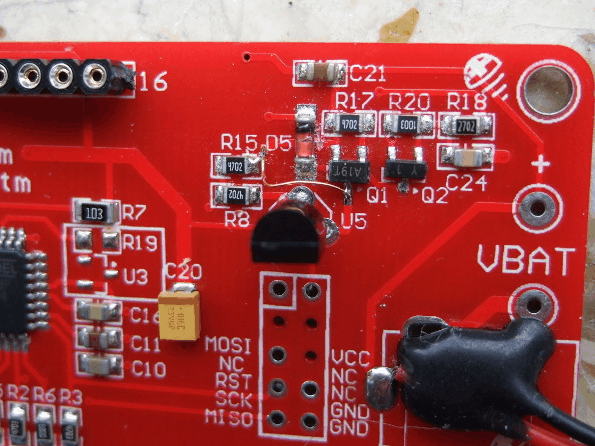
\includegraphics[width=12cm]{../PNG/Fish8840patch.png}
\caption{Picture of the changed Fish8840 printed board}
\label{fig:Fish8840patch}
\end{figure}

The scaling factor of the battery voltage must be specified in any case in the Makefile before any
attempt can be done to replace the original software (BAT\_NUMERATOR=66 for example).

The display module of the Fish8840 tester is equipped with a 3.3V voltage regulator to adapt
the operating voltage of the display controller.
Because the 3.3V operating voltage can be increased with the 5V signal level of the data signals
from the ATmega, a adapter circuit according to the picture \ref{fig:Fish8840Adapt} is recommended.
The four data signal lines are equipped with four serial \(2.7~k\Omega\) resistors at a little
breadboard.
Longer spacer bolts must be used to mount the display with the adapter board to the printed board
of the Fish8840 tester now.

\begin{figure}[H]
  \begin{subfigure}[b]{9cm}
    \centering
    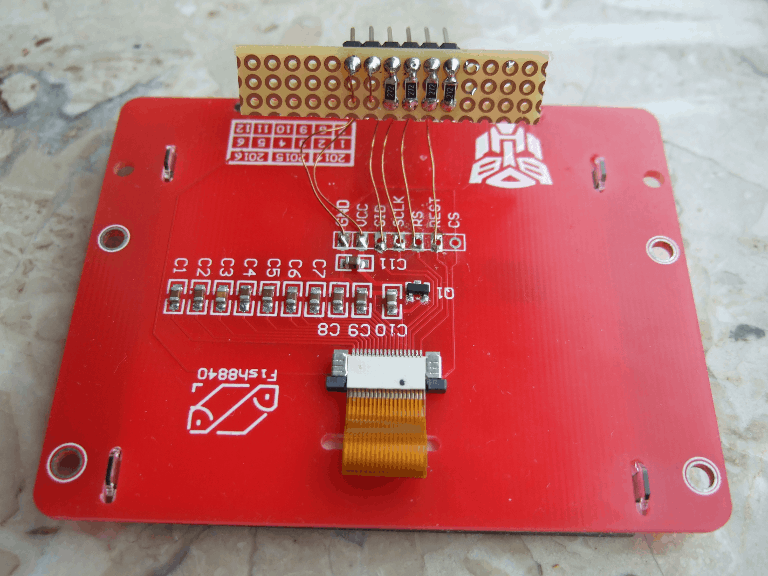
\includegraphics[width=9cm]{../PNG/Fish8840Adapt1.png}
    \caption{Display with the breadboard adapter}
  \end{subfigure}
  ~
  \begin{subfigure}[b]{9cm}
    \centering
    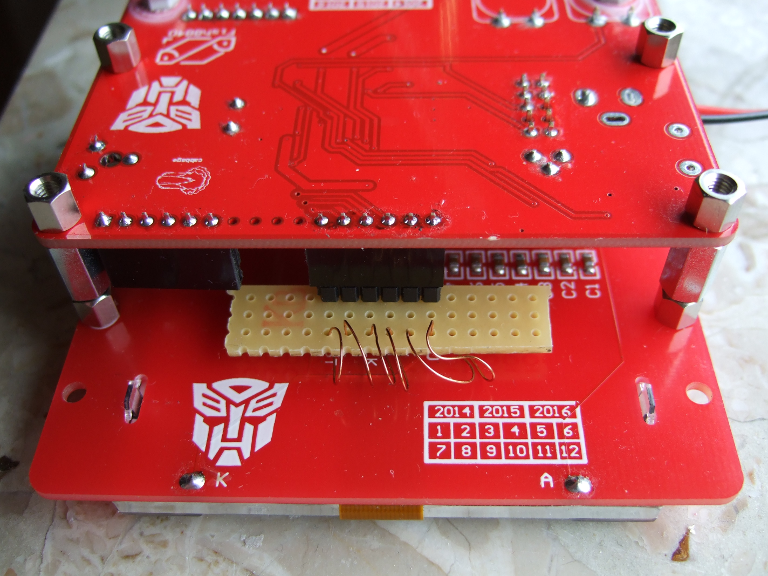
\includegraphics[width=9cm]{../PNG/Fish8840Adapt2.png}
    \caption{Ready mounted Tester}
  \end{subfigure}
  \caption{Adapter for a correctly display connection}
  \label{fig:Fish8840Adapt}
\end{figure}

All attempt to replace the original software is allways done at one's own risk.
No guaranty can be given for operational capability of newer software versions.
Unfortunately the original state of the chinese software can not be saved because the 
security bits of the ATmega328 are set. So there is no way to get back to the original state.

\section{Extented circuit with ATmega644 or ATmega1284}

A extended circuit for ATmega644/1284 processors was developed with Nick L. from the Ukraine.
The circuit \ref{fig:t644tester} enables a additional test of crystals and a extended range
for the frequency measurement.
Although the basic circuit is very simular to the circuit \ref{fig:ttester}, the
port assignment is different.
A rotary pulse encoder with circuit \ref{fig:RotExt} can be connected here at the pins PB5 and PB7 (instead of PD1 and PD3).
Both signals and also the power signals VCC and GND are available at the ISP connector,
so that the extension can also be connected here.\\

The 16:1 frequency divider of the 74HC4060 is allways used for frequencies above 2 MHz.
The frequency divider can also be used for frequencies between 25kHz and 400kHz to
upgrade the frequency resolution by using the period measurement.
For switching between the operational states (frequency divider and crystal oszillator)
the analog switches 74HC4052 are used.
The table \ref{tab:mega644-display} shows the pin assignments for the ATmega324/644/1284
microcontrollers for different display connections.
The using of the I\textsuperscript{2}C interface is only possible with the SSD1306 controller.
The signals of the I\textsuperscript{2}C interface require a pull-up resistor of \(4.7k\Omega\) to 3.3V.
The outputs of the ATmega is only switched to 0V for the I\textsuperscript{2}C signals.


\begin{table}[H]
  \begin{center}
    \begin{tabular}{| c || c | c | c | c |}
    \hline
      Port & Character LCD &  Graphik LCD  & Graphik LCD  & additional function\\
           &               &  SPI 4-wire   &   I\textsuperscript{2}C        &            \\
    \hline
    \hline
    PB2    &  LCD-RS         &            &             &       \\
    \hline
    PB3    &  LCD-E          &            &  LCD-SCL    &       \\
    \hline
    PB4    &  LCD-D4         &  LCD-REST  &  LCD-SDA    &       \\
    \hline
    PB5    &  LCD-D5         &  LCD-RS    &             & ISP-MOSI \\
           &                 &            &             & Rotary encoder 2 \\
    \hline
    PB6    &  LCD-D6         &  LCD-SCLK  &             & ISP-MISO \\
    \hline
    PB7    &  LCD-D7         &  LCD-SI    &             & ISP-SCK  \\
           &                 &            &             & Rotary encoder 1 \\
    \hline
    \end{tabular}
  \end{center}
  \caption{Different variations of the display port assignments}
  \label{tab:mega644-display}
\end{table}

You can also connect a display with the ST7108 controller ito the ATmega644 of ATmega1284 by using
a little circuit as shown in figure~\ref{fig:ST7108lcd_644}.
You should also respect the different pin assignments of display modules with ST7108 controllers as 
shown in table~\ref{tab:ST7108types} at page~\pageref{tab:ST7108types}.

\begin{figure}[H]
  \begin{subfigure}[b]{9cm}
    \centering
    
\includegraphics[width=8cm]{../FIG/ST7108serial164_644.eps}
    \caption{with 74HCT164}
  \end{subfigure}
  ~
  \begin{subfigure}[b]{9cm}
    \centering
    
\includegraphics[width=8cm]{../FIG/ST7108serial595_644.eps}
    \caption{with 74HCT595}
  \end{subfigure}
  \caption{Connection of a ST7108 Controller to a ATmega644/1284}
  \label{fig:ST7108lcd_644}
\end{figure}


\begin{figure}[H]
\centering

\includegraphics[width=18cm]{../FIG/t644tester.eps}
\caption{Extended Transistor Tester circuit with ATmega644}
\label{fig:t644tester}
\end{figure}


\section{Buildup of a tester with ATmega1280 or Arduino Mega}
The basic circuit of the tester can also be also build with a Arduino Mega with a ATmega1280
or ATmega2560 microcontroller with a shield.
The required connections are shown in figure~\ref{fig:t1280tester}.
The names for the connections of the display signals of the Arduino are shown with green color.
Components with red color identification are not required for operating.
The ATmega2560 controller has many connectors, but only one connector has the required
functions for both techniques of the frequency measurement.
The connector must be used as clock input for a build in counter and must also be 
used as interrupt source for change of signal level.
This feature is only available for the pin PE6 (T3/INT6).
The other clock inputs of counters PD7 (T0), PD6 (T1), PH7 (T4) and PL2 (T5) can not be 
used as interrupt source for status change.
Unfortunately the PE6 pin is not connected to a pin of the Arduino female connector strip.
The PE5 pin (7) is connected to the connector 3 of the PWM socket strip and
can be jumpered with the PE6 pin (8) of the ATmega2560.
The output signal of the frequency generation is available at the PB6 (OC1B) pin.
This pin is connected to the connector 12 of the PWM socket strip.
The ISP-connector is not required, because the program can be loaded with the bootloader
and the USB interface to the ATmega. With the bootloader there is always a
little delay for the power up start of the program.

\begin{figure}[H]
\centering

\includegraphics[width=18cm]{../FIG/t1280tester.eps}
\caption{TransistorTester circuit with ATmega1280, ATmega2560 or Arduino Mega}
\label{fig:t1280tester}
\end{figure}

Of course you can connect all supported displays also to the ATmega1280 or ATmega2560
as shown in table~\ref{tab:display-1280} .

\begin{table}[H]
  \begin{center}
    \begin{tabular}{| c || c | c | c | c | c | c |}
    \hline
           & Character     &  ST7565     & ST7920       & ST7108       & SSD1306     & Zusatzfunktion \\
      Port & LCD           &    SPI      & seriell      & seriell      &    I\textsuperscript{2}C      & \\
    \hline
    \hline
    PA0    &  LCD-D4       &   LCD-REST  &  LCD-RESET   & LCD-PCLK       &             & \\
    \hline
    PA1    &  LCD-D5       &   LCD-RS    &              & LCD-CS2        &             & Drehgeber-2 \\
    \hline
    PA2    &  LCD-D6       &   LCD-SCLK  &              & LCD-CLK        &             & \\
    \hline
    PA3    &  LCD-D7       &   LCD-SI    &              & LCD-CS1        &             & Drehgeber-1 \\
    \hline
    PA4    &  LCD-RS       &             &   LCD-B0     & LCD-B0 (RS)    &   LCD-SDA   & \\
    \hline
    PA5    &  LCD-E        &             &   LCD-EN     & LCD-EN         &   LCD--SCL  & \\
    \hline
    PA7    &  Tastensignal &             &              &                &             & \\
    \hline
    \end{tabular}
  \end{center}
  \caption{Connections for different display to the ATmega1280/2560 processors}
  \label{tab:display-1280}
\end{table}


\section{Programming of the microcontroller}
I release the software for the microcontroller with source code.
The developement is done with Linux operationg system (Ubuntu) and
is controlled with a Makefile. The Makefile makes shure, that your
software will be compiled with the prior selected Makefile options. Some constellations
are precompiled with the source. Please take a look to the ReadMe.txt file
in the directory Software/default and to the chapter~\ref{sec:config} at page~\pageref{sec:config}.
The result of compilation have the extensions .hex and .eep .
Usually the names will be TransistorTester.hex and TransistorTester.eep .
The .hex file contains the data for the program memory (flash) of the ATmega processor.
The .eep file contains the data for the EEprom memory of the ATmega. Both data files
must be loaded to the correct memory.

Additionally the operating state of the
ATmega processor must be programmed with the ``fuses''.
If you can use my Makefile and additionally the program avrdude \cite{avrdude}, you need no exact
knowledge of the details about the fuses. You have only to type ``make fuses'' if you
have no crystal or ``make fuses-crystal'' if you have installed the 8MHz crystal to your printed board.
With the ATmega168 series of the microcontroller you can also use ``make fuses-crystal-lp'' to use
a crytal with the low power mode.
Never choose the crystal mode of clock generation, if you don't have installed
the 8MHz crystal. If you are not shure with the fuses, leave them as default
set by manufactor and first bring the the tester to operation in this mode.
Maybe your program runs too slow, if you use program data compiled for
8MHz operation, but you can correct this later! But a wrong set of fuses may inhibit
later ISP-programming.

\subsection{Using the Makefile with Linux}
You can install packages with Debian based Linux versions by using a package manager as synaptic or dpkg.
The package ``subversion'' must be installed for downloading the sources or the documentation from the SVN archive.
With the command \\
``svn checkout svn://www.mikrocontroller.net/transistortester'' \\
you can download the complete archive.
Of course you can also download only subdirectories of the archive.
For using the Makefile in one of the subdirectories you must install the packages
make, binutils-avr, avrdude, avr-libc and gcc-avr.
Once you must prepare the access to the interfaces for the user.
If you open a consol window and you have also connected a ISP programmer with USB interface,
you can see the recognized USB devices with the command ''lsusb''.
A sample of the result of lsusb you can see here:
\begin{verbatim}
Bus 001 Device 001: ID 1d6b:0002 Linux Foundation 2.0 root hub
Bus 002 Device 003: ID 046d:c050 Logitech, Inc. RX 250 Optical Mouse
Bus 002 Device 058: ID 03eb:2104 Atmel Corp. AVR ISP mkII
Bus 002 Device 059: ID 2341:0042 Arduino SA Mega 2560 R3 (CDC ACM)
Bus 002 Device 001: ID 1d6b:0001 Linux Foundation 1.1 root hub
\end{verbatim}
A Device 58 is detected here a a AVR ISP mkII type (DIAMEX ALL-AVR).
The ID 03eb is a vendor ID and the ID 2104 is a product ID.
Both ID's are required for a entry in the file /etc/udev/ruled.d/90-atmel.rules .
In this example the file 90-atmel.rules has one line:
\begin{verbatim}
SUBSYSTEM=="usb", ATTRS{idVendor}=="03eb", ATTRS{idProduct}=="2104", MODE="0660",
GROUP="plugdev"
\end{verbatim}
This entry allow the access to the USB device 58 for members of the group ''plugdev''.
The also detected USB device 59 allows a access to the serial device ''/dev/ttyACM0'' for
members of the group ''dialout''.

Therefore your user identification should be a member of the group plugdev and also
a member of the group dialout.
With the command ''usermod -a -G dialout,plugdev \$USER'' the membership of both groups should be established.
Now the program avrdude should have permission to access both devices.
In a console window you must first change the directory with the command ``cd'' to a proper
subdirectory of the directory trunk.
Now you can change options of the Makefile with any text editor.
For compiling the source you must only type the simple command ``make''.
If the ISP programmer is configured proper in the Makefile, a command ``make upload''
should result to load the program with the ISP interface to the ATmega.
The ``fuses'' of the ATmega must also be set correctly once.
You can achieve this with the command ``make fuses'' or ``make fuses-crystal''.
The program avrdude probably reports a error for setting the extended fuse efuse.
The reading of unused fuse bits is specified as ''1'' for the ATmega, but the
avrdude program mask the unused bits, so that it expect a ''0'' for all unused bits.
Normally the efuse should be set to 0xfc, but avrdude read back 0x04 with the mask.
You can change the file avrdude.conf to change the behaviour of avrdude or
you can set the efuse to 0x04. 
The value for all efuses can be set with the identifier EFUSE\_VAL at the begin of file setup.mk
in the trunk directory.
Probably the fuses are also set correctly with the error message.

\subsection{Using the WinAVR package with Windows}
If you use the Windows operating system, the easiest way to get a correct programmed
ATmega is to use the WinAVR package \cite{winavr1},\cite{winavr2}.
With my patch \cite{winavr3} you can also set the fuses by using the Makefile.
Of course the avrdude program must support your programmer and the configuration
in the Makefile must match to your environment.

The figures \ref{fig:WinAVR1} show the File menu of the graphical user interface of WinAVR for
open the file Makefile and for saving the changed Makefile (Save).

\begin{figure}[H]
  \begin{subfigure}[b]{9cm}
    \centering
    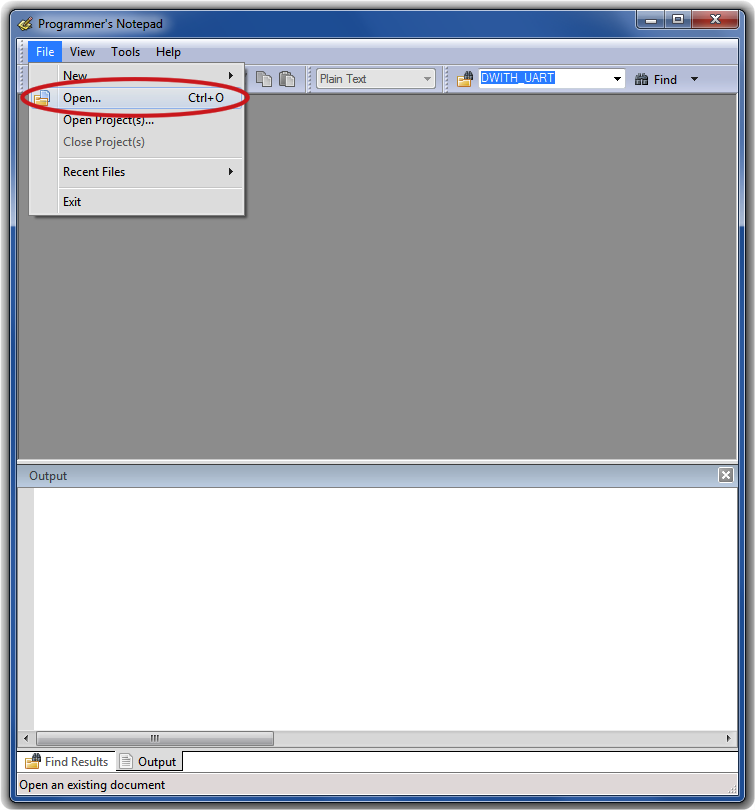
\includegraphics[width=9cm]{../PNG/Notepad_open.png}
    \caption{open Makefile}
  \end{subfigure}
  ~
  \begin{subfigure}[b]{9cm}
    \centering
    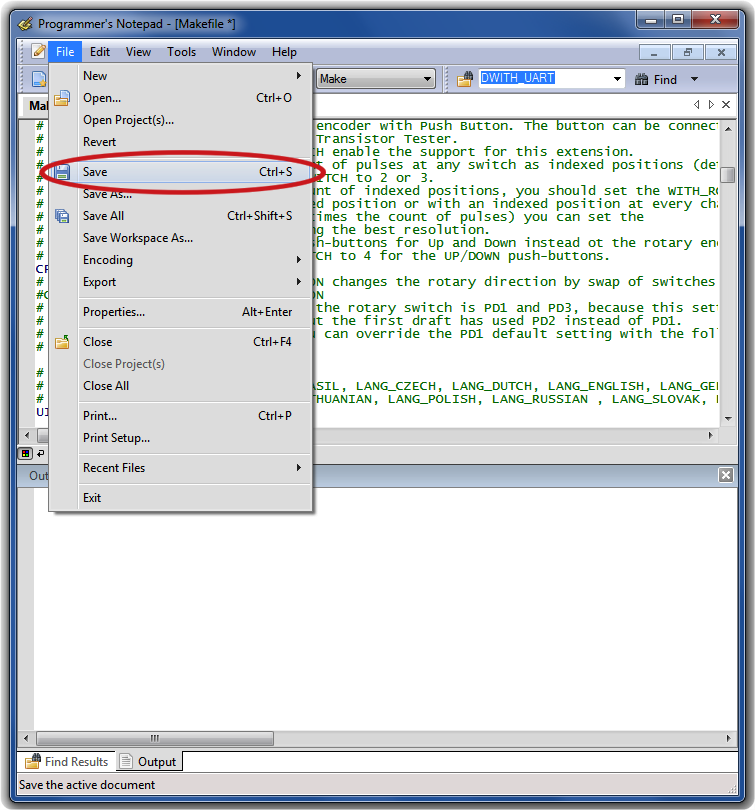
\includegraphics[width=9cm]{../PNG/Notepad_save.png}
    \caption{save Makefile}
  \end{subfigure}
  \caption{Using of the WinAVR user interface Programmer's Notepad}
  \label{fig:WinAVR1}
\end{figure}

The next figures \ref{fig:WinAVR2} show the Tools menu of the Programmer's Notepad
for compiling the program (Make All) and for programming the ATmega (Program) with avrdude.

\begin{figure}[H]
  \begin{subfigure}[b]{9cm}
    \centering
    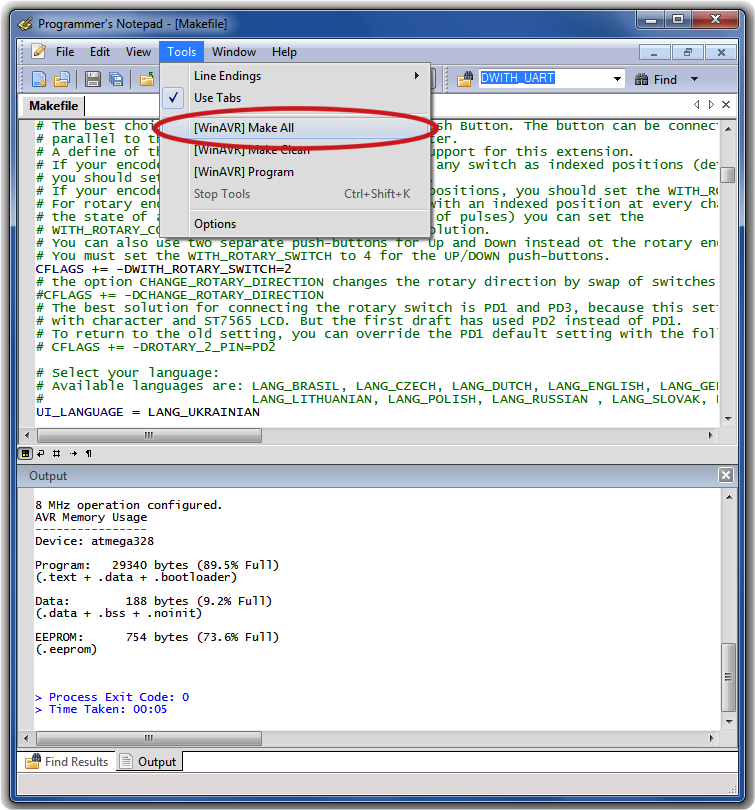
\includegraphics[width=9cm]{../PNG/Notepad_make.png}
    \caption{Build programming data (.hex/.eep)}
  \end{subfigure}
  ~
  \begin{subfigure}[b]{9cm}
    \centering
    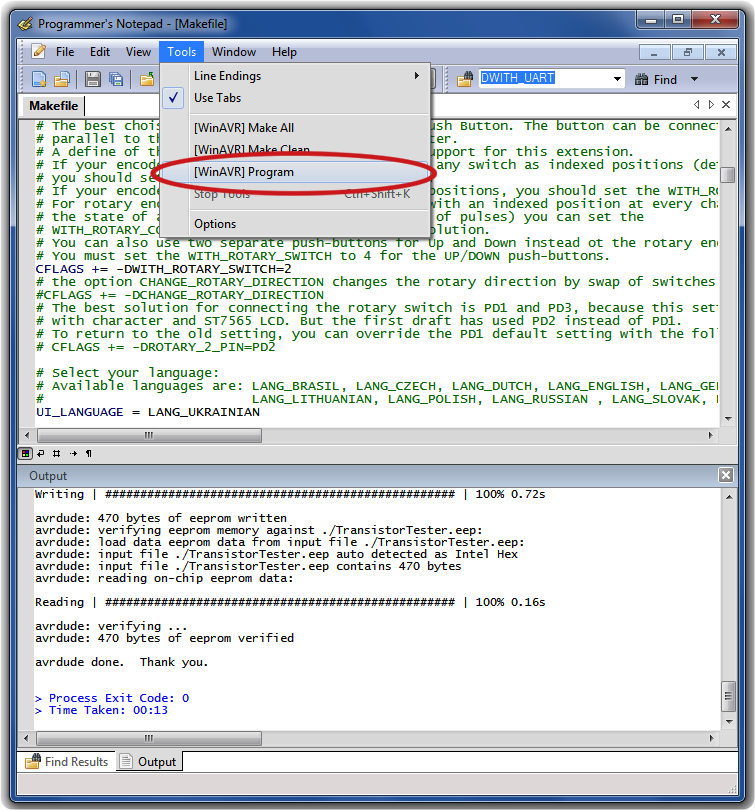
\includegraphics[width=9cm]{../PNG/Notepad_program.png}
    \caption{Programming the ATmega}
  \end{subfigure}
  \caption{Using of the WinAVR user interface Programmer's Notepad}
  \label{fig:WinAVR2}
\end{figure}



\section{Troubleshooting}
In most cases of problems you will miss the text output to the LCD-display.
At first you should check, if the LED was illuminated weak, if you release
the Test button. 
\begin{description}

\item[Power does not switch on.]
If the LED is without light and the VCC power has correct
5V voltage during holding the Test button, the microcontroller does not switch the power
correctly. The microcontroller should hold the power by switching the
PD6 output to 5V, which is usually done as one of the first actions.
If you hold the Test key pressed, the power is switched on anyway.
So you can check the value of VCC power and additionally the voltage value
of the PD6 output, if you hold the key pressed.
If VCC voltage has correct value (5V), but PD6 voltage is
below 4V, your microcontroller does not start the program. In this case
you should check if the microcontroller flash has been loaded with proper data for your
installed type and if ATmega is correctly configured with the fuses.
If your ATmega put the PD6 output to 5V and the power does not stay if you
release the Test key, it is more difficult to find the reason.
First you can shorten the LED and try again. If your Tester now starts,
your LED may be faulty or mounted with wrong polarity. If this is not
the reason, the current amplification factor of your T3 transistor (BC557C)
is insufficient. The current to the base of T3 is lower in the microcontroller
state as in the ``key pressed'' state.

\item[Nothing is readable on the LCD display]
Check the voltage at the contrast pin at the LCD display (pin 3). Adjust to
correct value specified in the data sheet of your display and optimize by viewing.
If you have a high temperature display type, you must provide a negative contrast voltage
for operation. In this case you can use the ICL~7660 device for generating
a negative voltage from positive 5V.

The tester software can be configured for many different controller with different connection
types. You should check, if your software matches to your mounted display type.
If there is no output readable on the LCD and the background light is on,
you should disconnect the power and check all four data plus the two control signal connections.
If all connection are well, the only reason I see is a uncorrect timing of
control signals. This can be caused by a slower LCD controller than expected by
the software or the ATmega software runs at wrong clock speed. Please check for which
clock speed your programming data was compiled  and if the fuses of the
ATmega are correct set to that speed. You find the clock parameter in the corresponding
Makefile.
If the tester is build without the switch off electronic, you can test with
a LED connected to the test pins, if the program operates normally.
If the LED flickers, the program operates well. The missing text on the
LCD must be caused by wrong connection or timing.
For some graphical displays the contrast is changeable with a menu function.
If you have changed the contrast value, that nothing is readable at the screen,
you cannot handle the menu function any more. You can try to read the display
from a slanting look to the display, not from the front side.
In this case you can try to handle the menu function with this view.
Otherwise you can write the EEprom data new with a ISP programmer to reset the contrast value.


\item[Something but not all is readable on the LCD display]
Check if the .eep data are loaded to the EEprom memory of ATmega.
If all data are loaded correctly, you should check the clock speed of your
programming data (Makefile) and ATmega processor settings (fuses).

\item[Measurement is slow and Capacitors are measured about 8 times too small]
You run software compiled for 8MHz clock at real clock speed of 1MHz.
Please set the fuses of the ATmega correctly.

\item[Measurement has strangely values]
Check if your programmer is still connected to the ISP-plug.
The ISP interface should be disconnected for measuring.
Very often the reason of wrong measurements is the use of software compiled with
the AUTOSCALE\_ADC option and with the option NO\_REF\_CAP, but the capacitor
at the AREF pin has still a value of 100nF.
Wrong assembly of components or remaining soft solder flux can disturb the 
measurements too. Please check with the selftest function of your TransistorTester software
if possible. For the details see Chapter \ref{sec:selftest}.

Otherwise inspect your board visually and check the resistor values
with a ohmmeter. You can use the pins of the ATmega for this check, for example
to check the R1 you can measure between pin 23 and pin 14. Take a look at the
circuit diagram \ref{fig:ttester} for details. There is no need to
remove the microcontroller, only battery or power supply should be removed before.

\item[The Tester switch off the power after 2 seconds display time] 
This condition exists, if the external Pull-Up resistor at the PD7 input
is missing or the key button is keep pressed.
The software switch off the internal Pull-Up resistors to prevent a influence
to the measurement results. Therefore a external Pull-Up resistor (27k) is required.

\item[Der Tester shows only Vext=xx.xV in row 2]
This problem exists, if the Pull-Up resistor at the PD7 input
is missing or the key button is keep pressed.
Additionally the software is configured without the serial output (without option WITH\_UART) and
without the internal Pull-Up resistors (with option PULLUP\_DISABLE).
You should install the Pull-Up resistor at pin PD7.


\end{description}
